\chapter{Tabular models} \label{ch:tabular}
\begin{NoteBox}
At present we allow only three independent variables in \Vaango.
\end{NoteBox}

MPM tabular material data is often of the form  shown in Figure~\ref{fig:tabular_data}.
In this particular data set, we have three independent variables: the plastic strain ($\beta$),
the saturation ($\alpha$), and the strain ($\Veps$).  Pressure ($p$) is the dependent variable.
The data represents a function of the form $p = p(\Veps, \alpha, \beta)$.  We are given 
an input point in the three-dimensional independent variable space, 
($\Veps_0$, $\alpha_0$, $\beta_0$), and we would like to find the corresponding value of
the pressure, $p_0$.
\begin{figure}[htbp!]
  \centering
  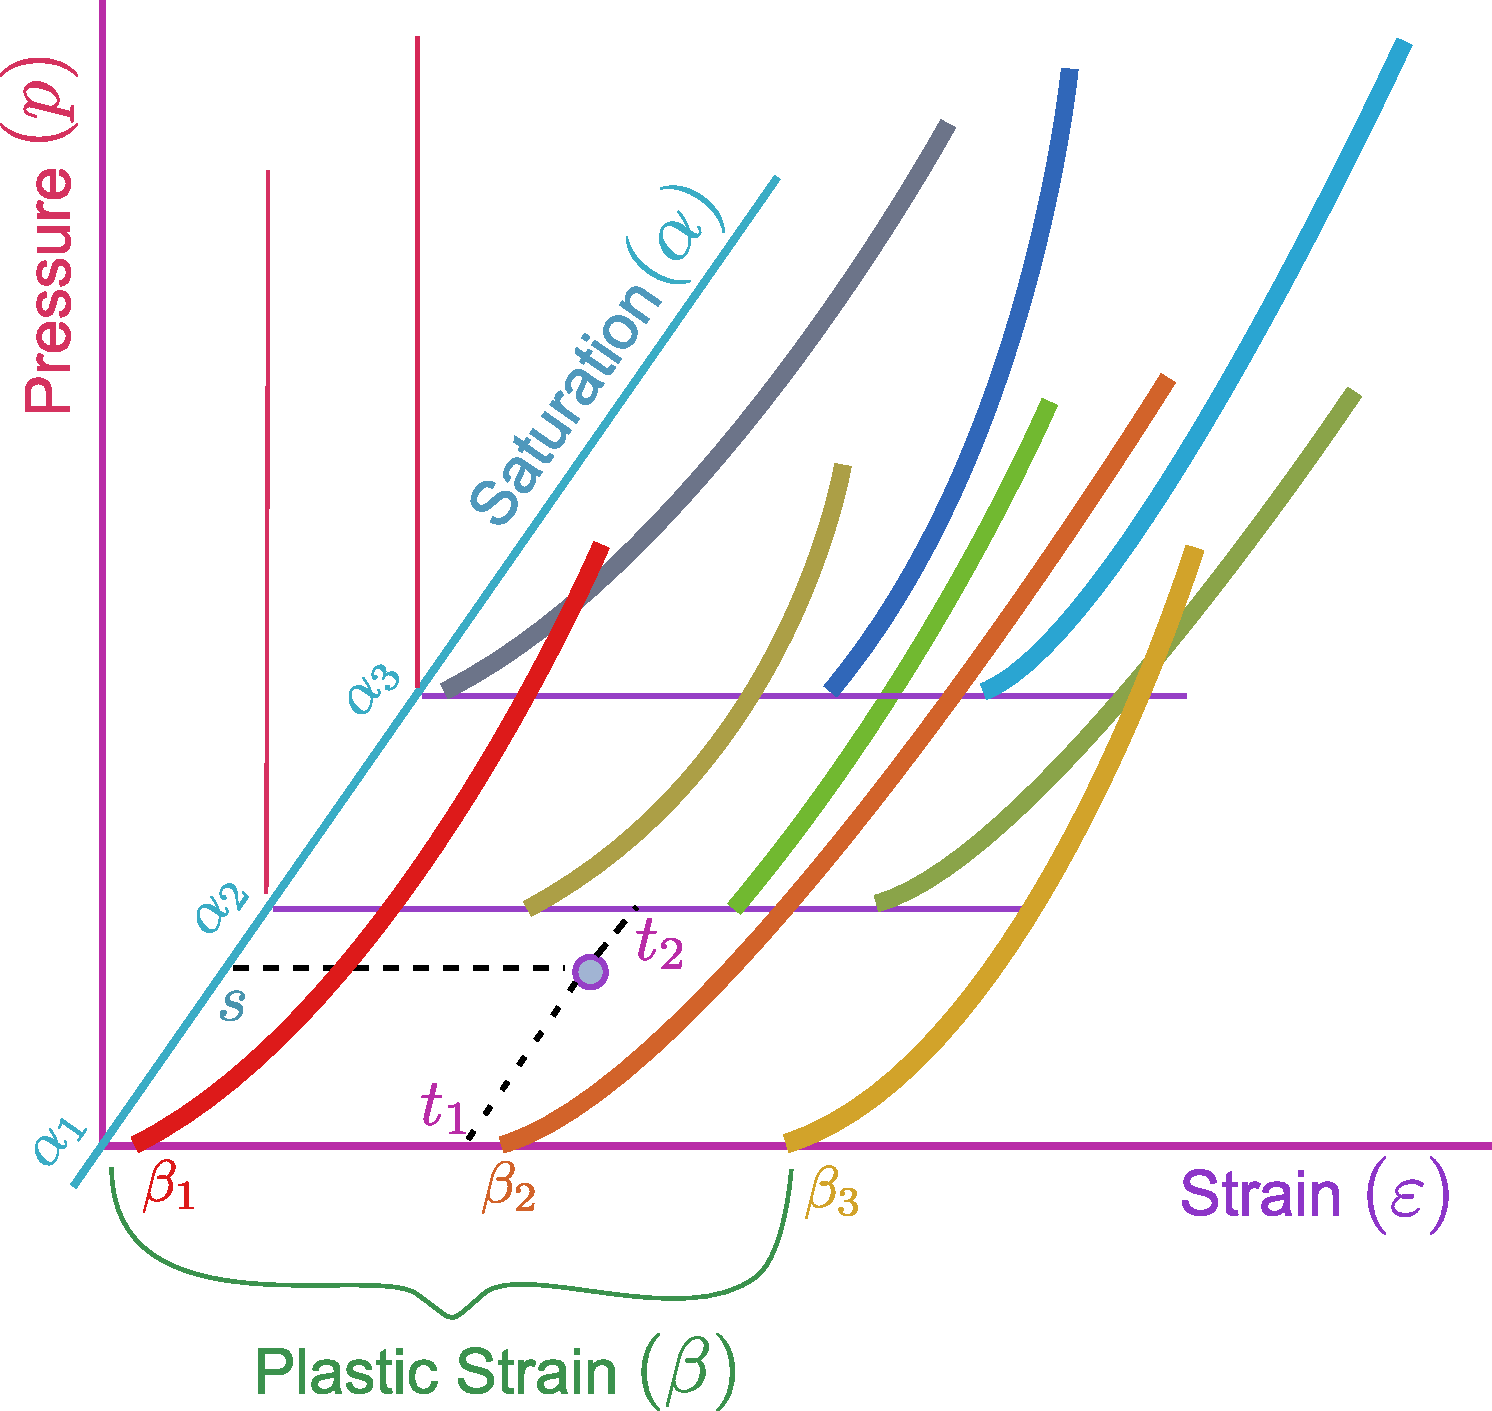
\includegraphics[width=0.5\textwidth]{Figs/tabular/table_interpolation.pdf}
  \caption{Schematic of tabular material data for MPM constitutive models. The circle
           in blue is the input data point for which we would like to find the pressure.}
  \label{fig:tabular_data}
\end{figure}

As we can see from the figure, the data are largely unstructured.  However, there is
some structure to the data.  For instance, the data are provided for three values of
saturation, $[\alpha_1, \alpha_2, \alpha_3]$.  For each value of $\alpha$, we have 
data for a few plastic strain values: $\alpha_1$ : $[\beta_{11}, \beta_{12}, \beta_{13}]$,
$\alpha_2$ : $[\beta_{21}, \beta_{22}, \beta_{23}, \beta_{24}, \dots]$, and
$\alpha_3$ : $[\beta_{31}, \beta_{32}, \dots]$.  Finally, for each value of the plastic
strain, we have a pressure-strain curve, for example, for
$\alpha_1, \beta_{11}$ : $[\Veps_{111}, \Veps_{112}, \Veps_{113}, \dots, \Veps_{11N}]$ and
$[p_{111}, p_{112}, p_{113}, \dots, p_{11N}]$, or for
$\alpha_3, \beta_{32}$ : $[\Veps_{321}, \Veps_{322}, \Veps_{323}, \dots, \Veps_{32M}]$ and
$[p_{321}, p_{321}, p_{321}, \dots, p_{32M}]$.  Clearly, the data become quite complex
as the number of dimensions is increased.  


\section{Linear interpolation}
\begin{NoteBox}
The procedure below assumes that the $\alpha$ values are sorted in ascending order.
If $\alpha_0 \notin [\alpha_1, \alpha_N]$, \Vaango will throw an exception and
exit.  Also observe that at least two sets of data are needed for the interpolation
procedure to work.
\end{NoteBox}

In this section we describe the process used in \Vaango to interpolate the data.
For simplicity, we only consider two independent variables, the saturation ($\alpha$)
and the strain ($\Veps$) as shown in Figure~\ref{fig:tabular_data_step1}.  
\begin{figure}[htbp!]
  \centering
  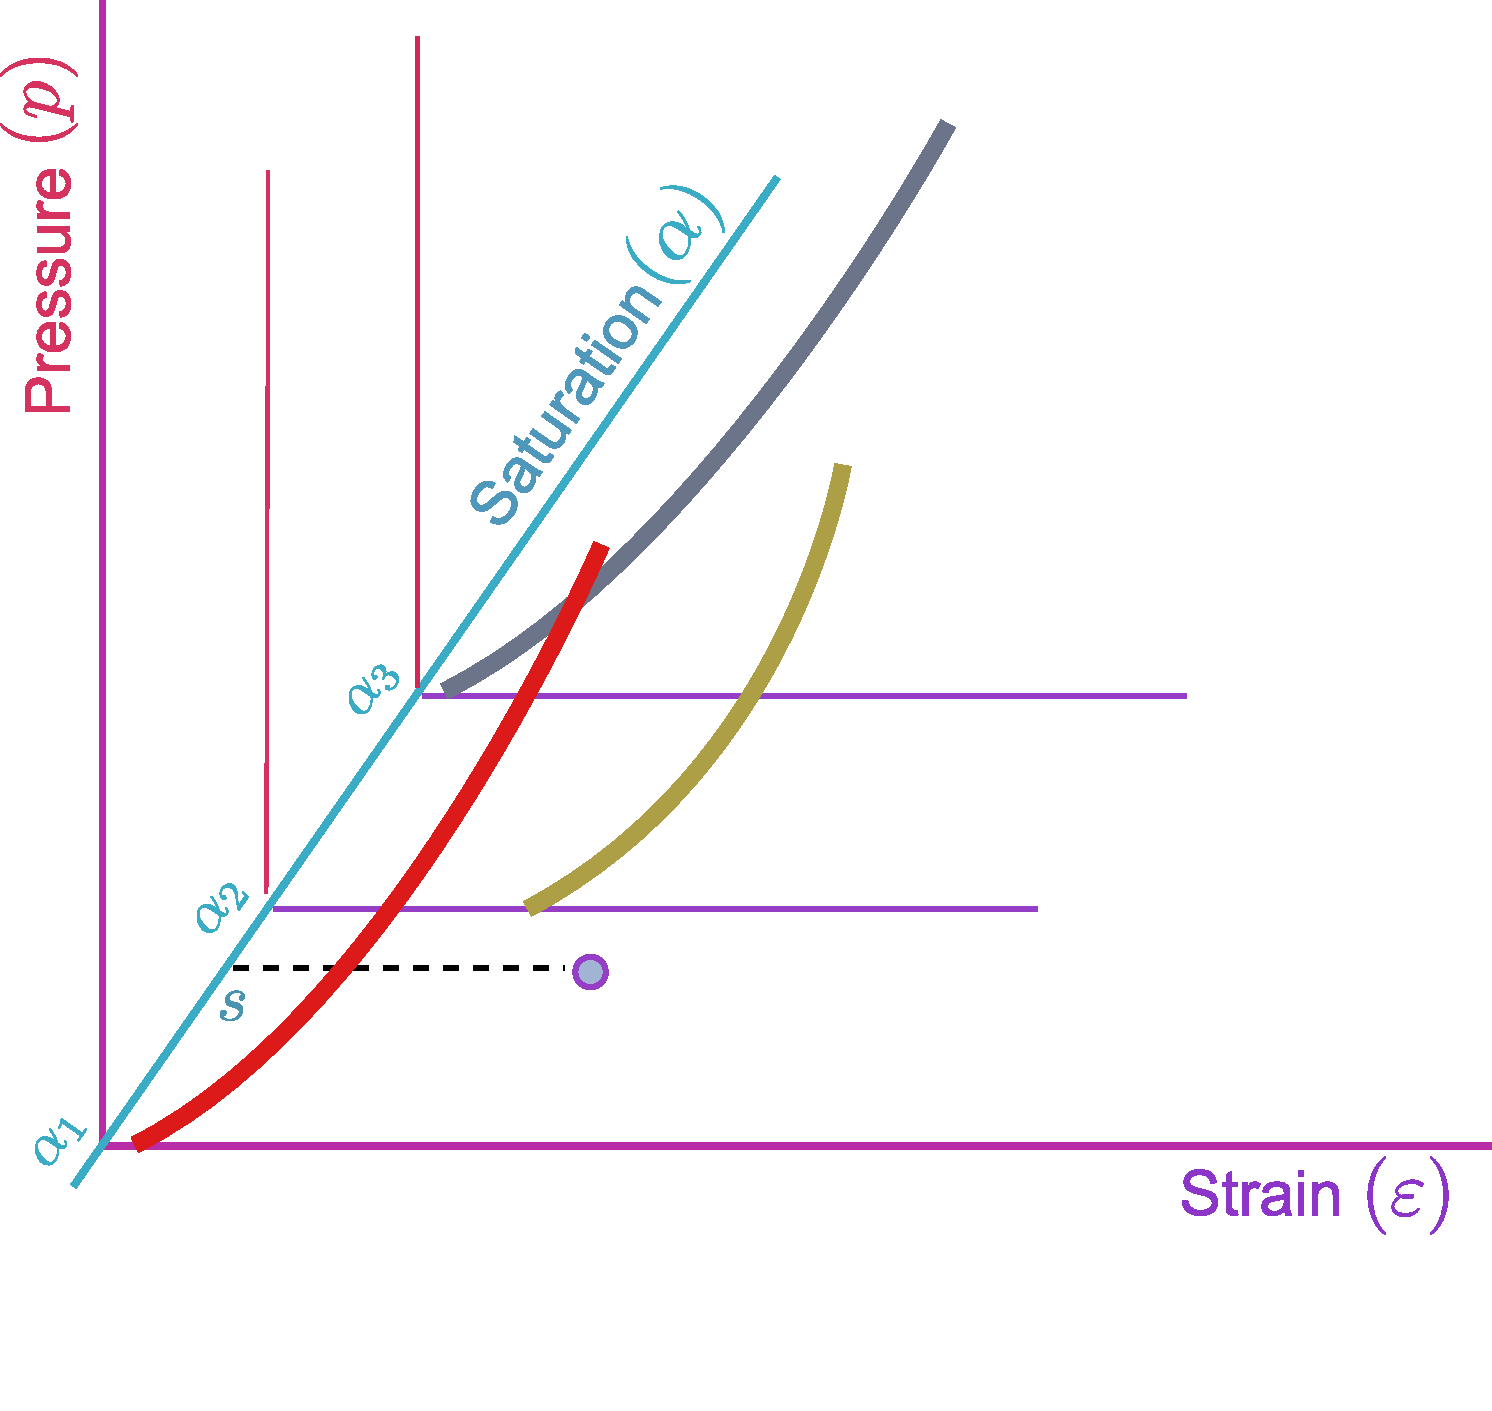
\includegraphics[width=0.5\textwidth]{Figs/tabular/table_interpolation_step1.pdf}
  \caption{Schematic of a three variable table of material data. The 
           circle in blue is the input point for which we would like to find the pressure.}
  \label{fig:tabular_data_step1}
\end{figure}

The first step in the process is to find the pressure-strain data that are needed 
for the interpolation process.  This can be accomplished by iterating through 
the $\alpha$s and finding a value of the parameter $s \in [0,1]$ where
\Beq
  s = \frac{\alpha_0 - \alpha_k}{\alpha_{k+1} - \alpha_k}~,~~ k=1,2,\dots,N-1
\Eeq
where $N$ is the number of values of $\alpha$ for which data area available.


Once the two curves needed for interpolation have been identified, the next step is
to find the segments of the pressure-strain curves that correspond to the input
variable $\Veps_0$.  These segments are highlighted with thick lines in 
Figure~\ref{fig:tabular_data_step2}.  The two associated parameters $t_1$ and $t_2$
are calculated using
\Beq
  \Bal
  t_1 &= \frac{\Veps_0 - \Veps_{j,k}}{\Veps_{j,k+1} - \Veps_{j,k}}~,~~ k=1,2,\dots,M_j-1 \\
  t_2 &= \frac{\Veps_0 - \Veps_{j+1,k}}{\Veps_{j+1,k+1} - \Veps_{j+1,k}}~,~~ k=1,2,\dots,M_{j+1}-1
  \Eal
\Eeq
where $\Veps_{j,k}$ is a point on the pressure-strain curve for saturation $\alpha_j$, 
and $M_j$ is the number of points on the curve.
\begin{figure}[htbp!]
  \centering
  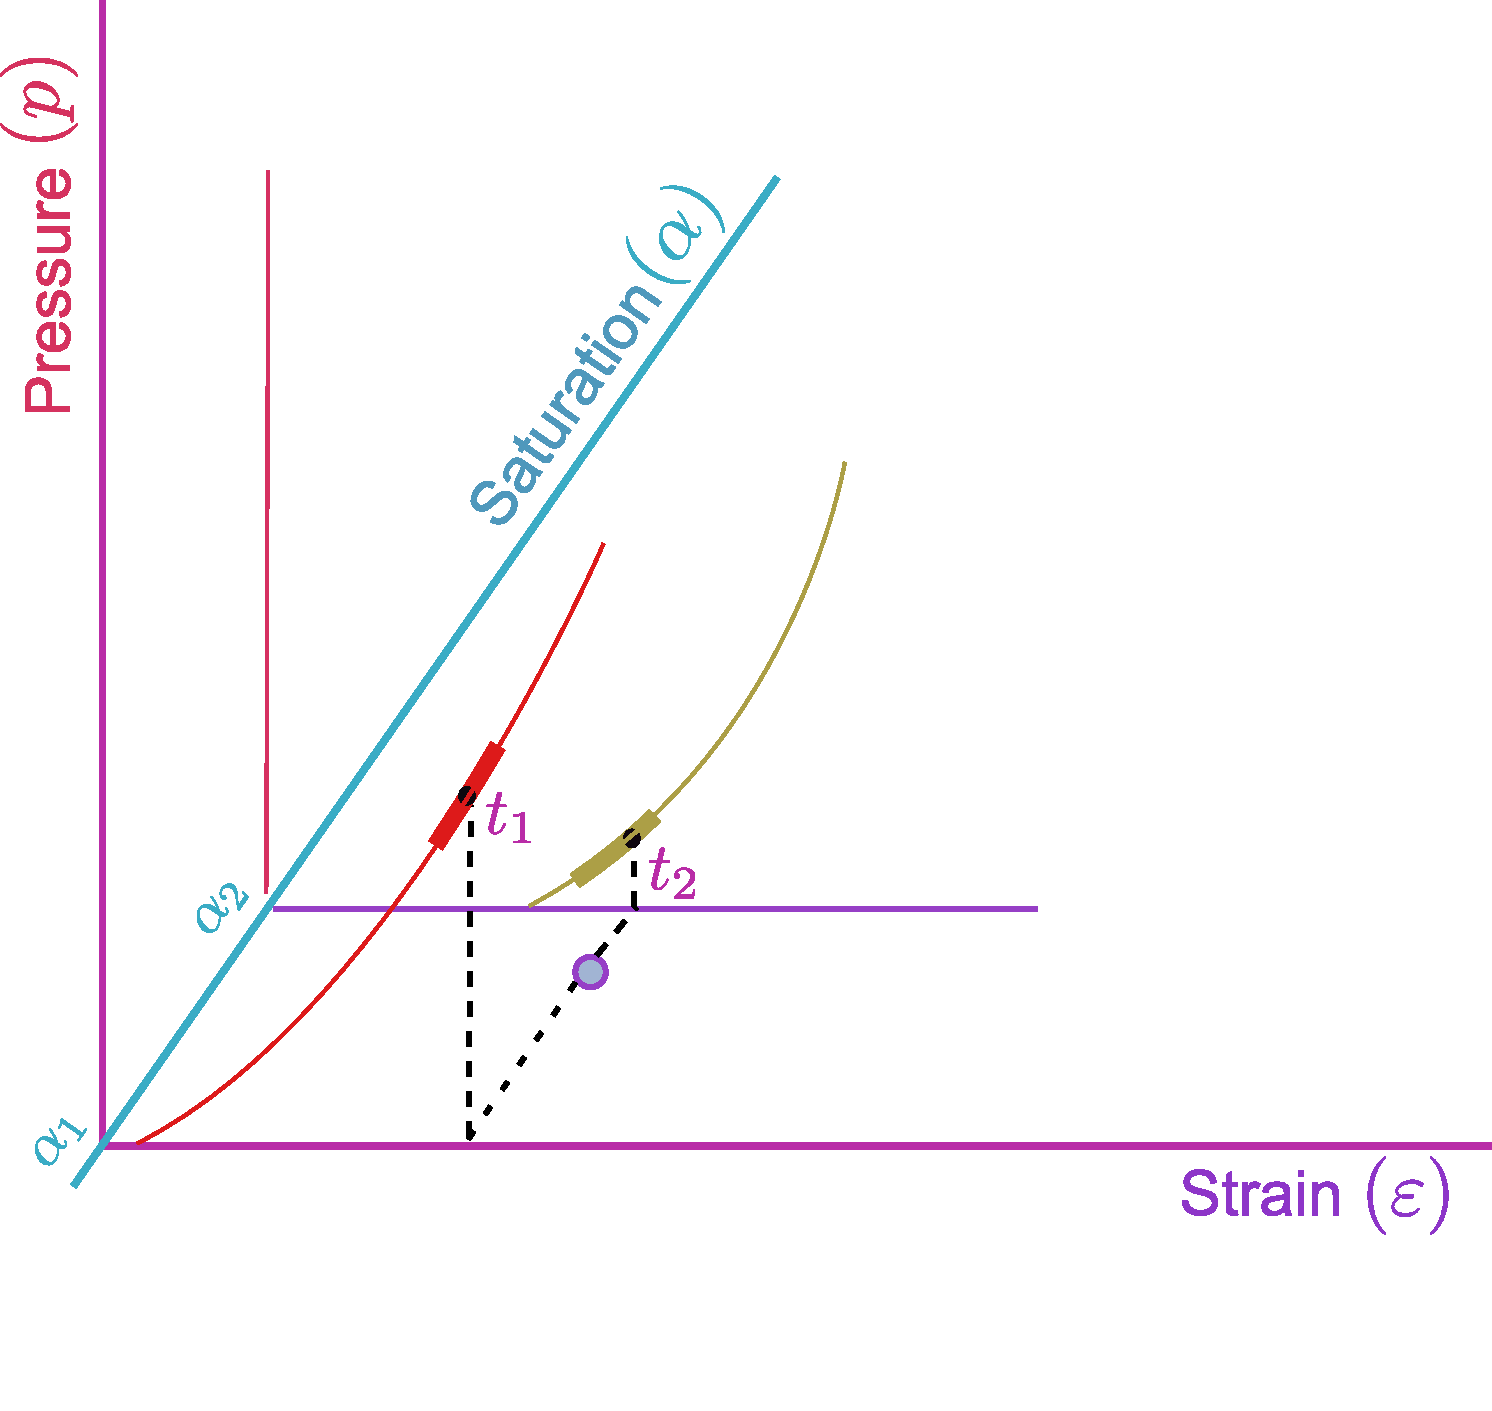
\includegraphics[width=0.5\textwidth]{Figs/tabular/table_interpolation_step2.pdf}
  \caption{Second stage of interpolation of a three variable table of material data. The 
           circle in blue is the input point for which we would like to find the pressure.}
  \label{fig:tabular_data_step2}
\end{figure}

We can now compute the pressures at these two points, using
\Beq
  \Bal
    p_1 &= (1 - t_1) p_{j,k} + t_1 p_{j,k+1} \\
    p_2 &= (1 - t_2) p_{j+1,k} + t_2 p_{j+1,k+1}
  \Eal
\Eeq
The final step of the process is to compute the interpolated pressure $p_0$ using
\Beq
  p_0 = (1 - s) p_1 + s p_2 \,.
\Eeq
A schematic of this operation is shown in Figure~\ref{fig:tabular_data_step3}.
\begin{figure}[htbp!]
  \centering
  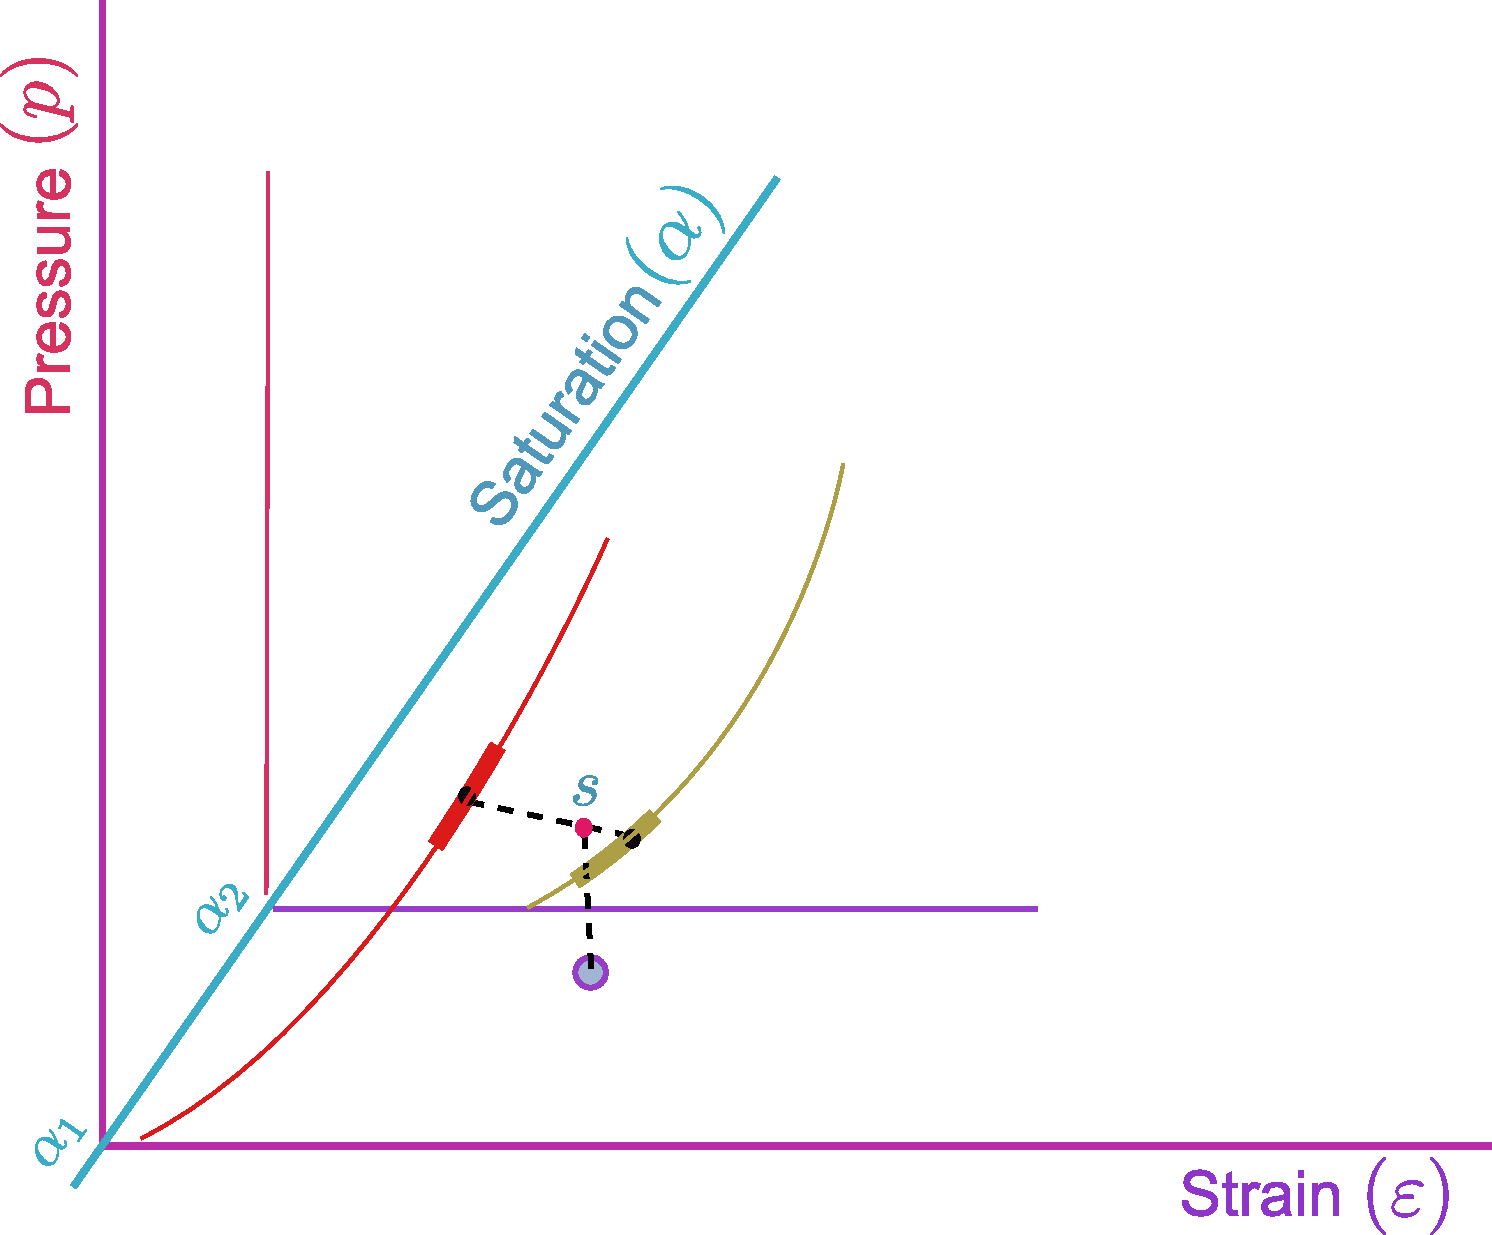
\includegraphics[width=0.5\textwidth]{Figs/tabular/table_interpolation_step3.pdf}
  \caption{Final stage of interpolation of a three variable table of material data. The 
           circle in blue is the input point and the red circle is the interpolated value.}
  \label{fig:tabular_data_step3}
\end{figure}

\section{The tabular equation of state}
For the tabular equation of state, we assume that there is only one independent variable,
the density ratio $\eta = \rho/\rho_0$ where $\rho$ is the current mass density and $\rho_0$ is
its reference value.  The dependent variable is the pressure, $\pbar = \pbar(\eta)$, which is
positive in compression.  A linear interpolation is done to compute the pressure
for a given state of deformation.

The bulk modulus is computed using
\Beq
  K = \rho \left[\frac{p(\eta +\epsilon) - p(\eta-\epsilon)}{2\epsilon}\right]
\Eeq
\begin{WarningBox}
The tolerance $\epsilon$ is hardcoded to $10^{-6}$ in \Vaango but
may not be adequate for some problems.
\end{WarningBox}

\section{The tabular plasticity model}
The tabular plasticity model was designed for materials that have almost no tensile strength, and
the inputs are expected in the \textbf{compression positive} convention.  Note that the general
convention used in the Vaango code is that \textbf{tension is positive and compression is negative}.
Conversions are done internally in the code to make sure that signs are consistent.

The model uses isotropic elasticity, with a shear modulus that is either a constant ($G_0$) or 
determined using a Poisson's ratio ($\nu$) from the tabular bulk modulus, $K(p)$:
\Beq
  G = \frac{3K(1-2\nu)}{2(1+\nu)}
\Eeq
This relation is activated if $\nu \in [-1.0, 0.5)$, otherwise the constant shear modulus
is used.

The tangent bulk modulus is determined from a table of unloading curves (see 
Figure~\ref{fig:tabular_unload_curves} of the mean stress, $\pbar$, as a function
of the total Hencky volumetric strain, $\bar{\Veps_p}$.  Each unloading 
curve is associated with a Hencky plastic volumetric strain ($\bar{\Veps_v^p}$).
Additive decomposition of the volumetric strains is assumed.  The plastic volumetric 
strain is subtracted from the total volumetric strain to compute the elastic
volumetric strain ($\bar{\Veps_v^e}$).  The data stored in the table is therefore
of the form $\pbar(\bar{\Veps_v^p},\bar{\Veps_v^e})$ and the bulk modulus is computed,
after interpolation, using the central difference scheme:
\Beq
  K(\bar{\Veps_v^p}_0, \bar{\Veps_v^e}_0) = 
    \frac{p(\bar{\Veps_v^p}_0, \bar{\Veps_v^e}_0 +\epsilon) 
       - p(\bar{\Veps_v^p}_0, \bar{\Veps_v^e}_0-\epsilon)}{2\epsilon}
\Eeq
\begin{WarningBox}
The tolerance $\epsilon$ is hardcoded to $10^{-6}$ in \Vaango and
may not be adequate for some problems.
\end{WarningBox}
\begin{figure}[htbp!]
  \centering
  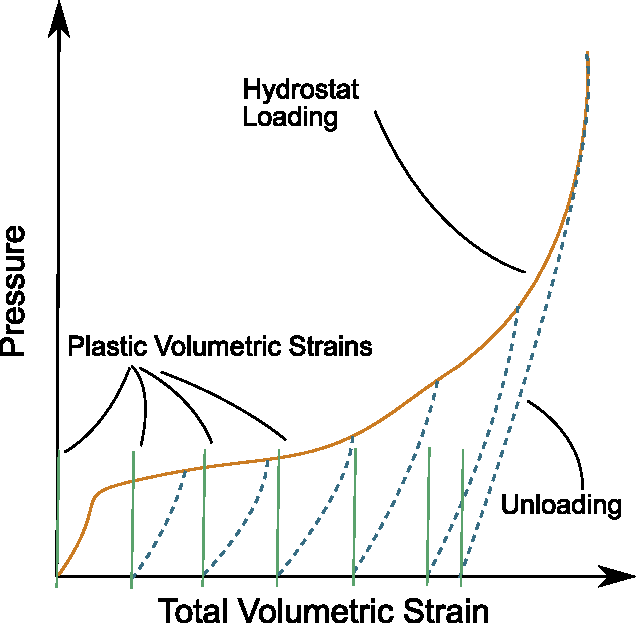
\includegraphics[width=0.5\textwidth]{Figs/tabular/TabularHydrostat.pdf}
  \caption{Unloading curves uses to determine the tangent bulk modulus for the
           tabular plasticity model at various plastic strain value.}
  \label{fig:tabular_unload_curves}
\end{figure}

The tabular yield condition has the form
\Beq
  f = \sqrt{J_2} - g(\pbar) = 0
\Eeq
The function $g(\pbar)$ is provided in tabular form and is depicted in 
Figure~\ref{fig:tabular_yield_function}(a). 
To ensure convexity of the tabular data, a convex hull of the data points is computed
first as shown in Figure~\ref{fig:tabular_yield_function}(b).
\begin{figure}[htbp!]
  \begin{subfigure}[t]{0.5\textwidth}
    \centering
    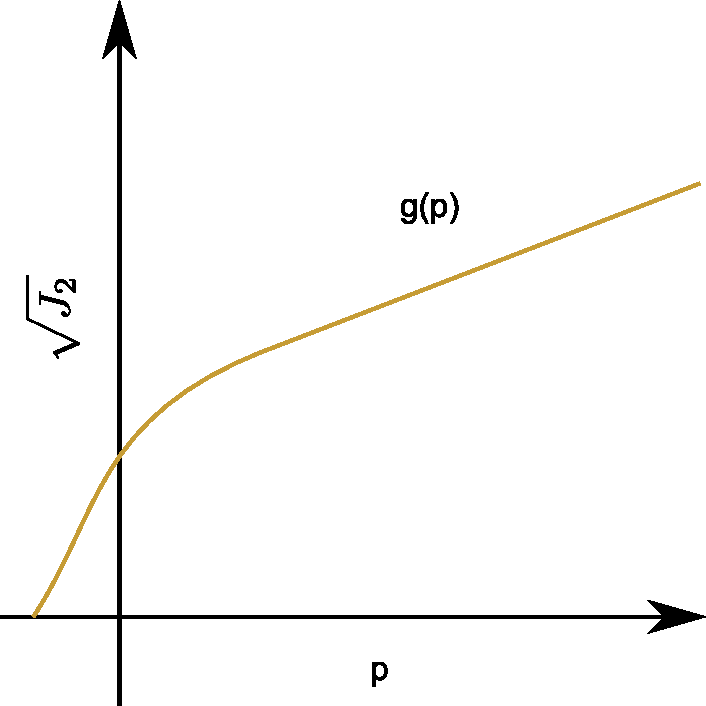
\includegraphics[width=\textwidth]{Figs/tabular/TabularYieldFn.pdf}
    \caption{Yield function}
  \end{subfigure}
  \begin{subfigure}[t]{0.5\textwidth}
    \centering
    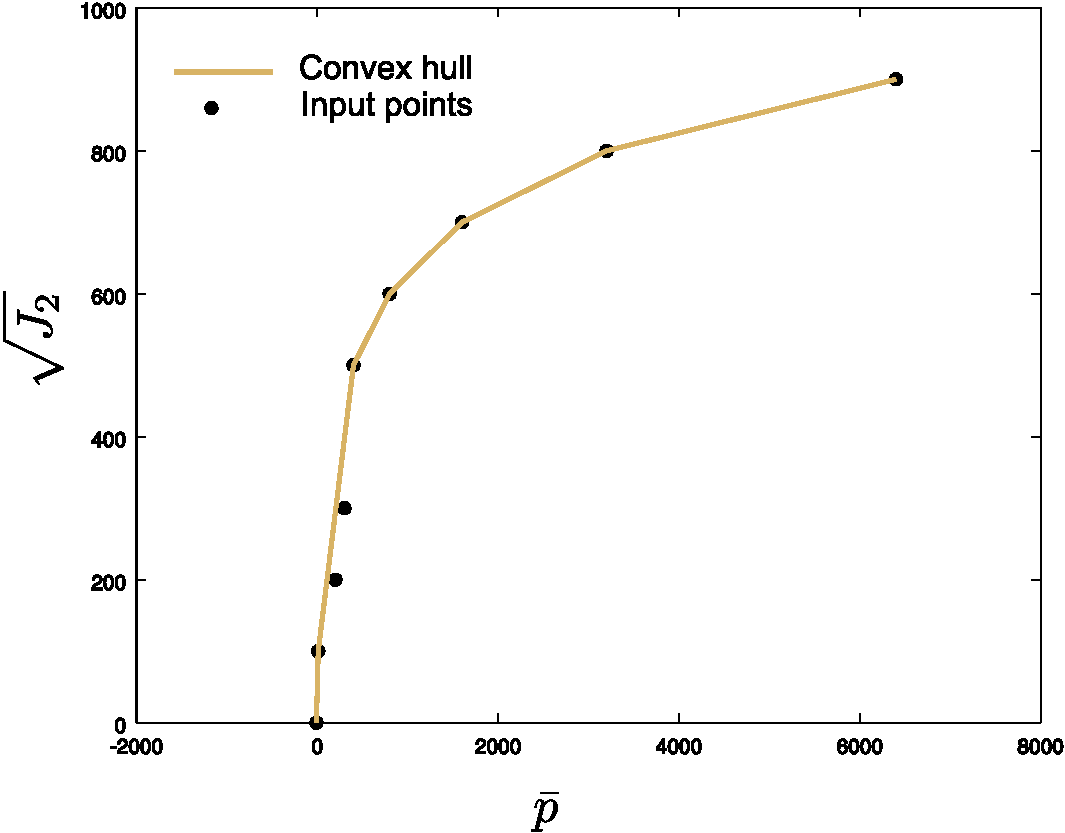
\includegraphics[width=\textwidth]{Figs/tabular/tabular_yield_hull.pdf}
    \caption{Computed hull of the input data}
  \end{subfigure}
  \caption{Yield function used by the tabular plasticity.}
  \label{fig:tabular_yield_function}
\end{figure}

Linear interpolation is used to determine is a stress state is inside the yield
surface.  We also compute a normal to the yield surface using linear interpolation
and a central difference scheme (similar to that used to compute the bulk modulus).
However, the actual return algorithm uses a geometric closest point computation
rather than the derivative of the yield function with respect to the stress. The
approach is similar to that used in the \Arena material model.

If the number of points in the input table is equal to 2, the yield function is
either a von Mises model or a linear Drucker-Prager model.  In that can we find
the closest point to the tabular data directly.

For tables with more than two input points, we fit a quadratic B-spline to the
closest segment of the input tabular data and find the closest distance to that
spline.  Approximating, rather than interpolating, splines are used to retain 
the convexity of the yield function.

The B-splines are computed using
\Beq
  s_x = \Ba \cdot (\BM_j \cdot \Bp_x) ~,~~
  s_y = \Ba \cdot (\BM_j \cdot \Bp_y)
\Eeq
where $\Ba = (1, t, t^2)$, $t \in [0,1]$ parameterizes each segment of the tabular data,
$\Bp_x = (x_k, x_{k+1}, x_{k+2})$, $\Bp_y = (y_k, y_{k+1}, y_{k+2})$, 
and $(x_k, y_k)$ are the input $0, \dots, N-1$ tabular data points.
The associated matrices that are used are:
\Beq
  \BM_{j=0} = 0.5 \begin{bmatrix} 2 & 0 & 0 \\ -4 & 4 & 0 \\ 2 & -3 & 1 \end{bmatrix} ~,~~
  \BM_j = 0.5 \begin{bmatrix} 1 & 1 & 0 \\ -2 & 2 & 0 \\ 1 & -3 & 2 \end{bmatrix} ~,~~
  \BM_{j=N-1} = 0.5 \begin{bmatrix} 1 & 1 & 0 \\ -2 & 2 & 0 \\ 1 & -2 & 1 \end{bmatrix}
\Eeq

Closest point projections of stress states outside the yield surface to fitted B-splines 
along the yield surface are shown in Figure~\ref{fig:tabular_yield_closest}.
\begin{figure}[htbp!]
  \begin{subfigure}[t]{0.5\textwidth}
    \centering
    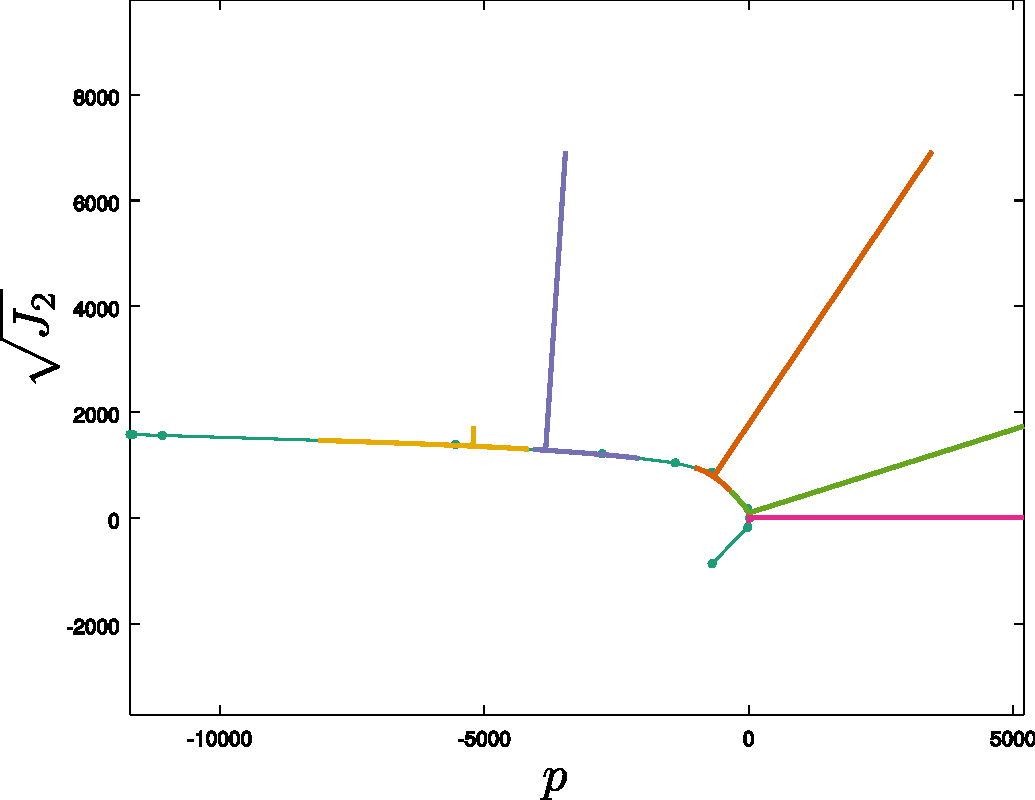
\includegraphics[width=\textwidth]{Figs/tabular/table_yield_closest.pdf}
    \caption{Closest points to yield function}
  \end{subfigure}
  \begin{subfigure}[t]{0.5\textwidth}
    \centering
    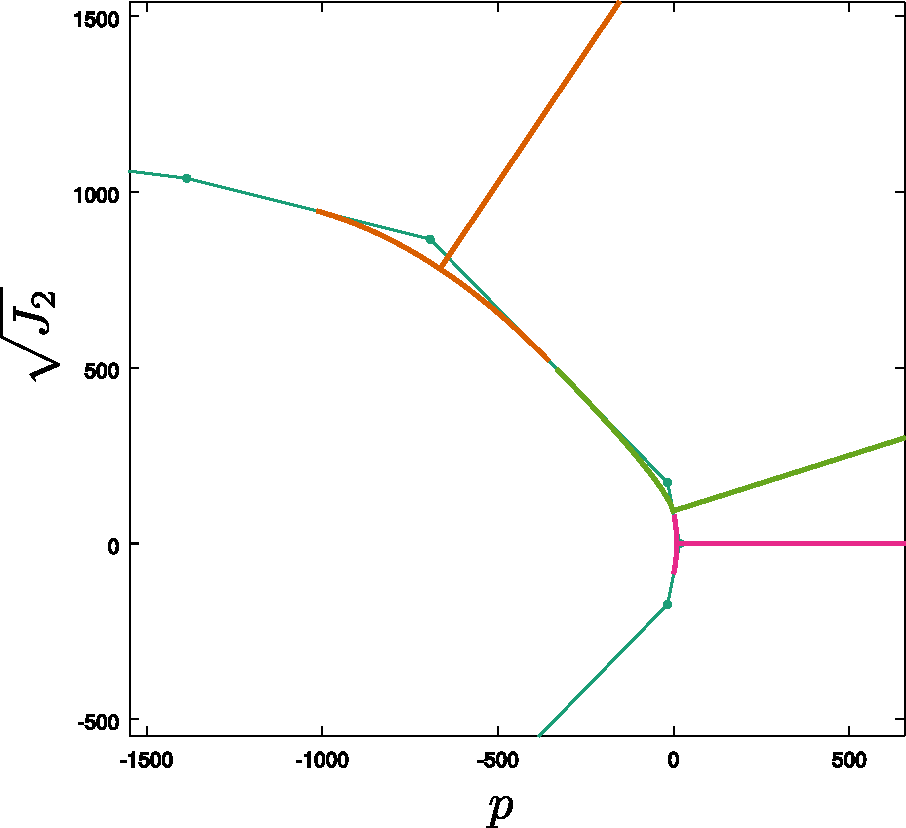
\includegraphics[width=\textwidth]{Figs/tabular/table_yield_closest_zoom.pdf}
    \caption{Zoomed view showing B-splines}
  \end{subfigure}
  \caption{Closest point projections to yield function used by the tabular plasticity.}
  \label{fig:tabular_yield_closest}
\end{figure}

\section{Theory behind closest-point projection}
The ideas behind the closest-point projection approach were made rigorous in the
mid-to-late 1980s by a group of researchers influenced by developments in convex optimization. 

\subsection{ Background }
In nonlinear optimization, the method of Lagrange multipliers has been used since the mid 1800s to solve minimization problems with *equality* constraints.  In
1950, this approach was generalized by Kuhn and Tucker to allow for *inequality* constraints.  Later it was discovered that W. Karush from the University of Chicago had reached the same conclusions in his MSc thesis from 1939.

\subsubsection{ Primal form  }
The primal form of the optimization problem is
\Beq
  \begin{aligned}
    & \text{minimize}   & & f(\mathbf{x}) \\
    & \text{subject to} & & g_i(\mathbf{x}) \le 0, \quad i = 1, \dots, m \\
    &                   & & h_j(\mathbf{x}) = 0, \quad j = 1, \dots, p 
  \end{aligned}
\Eeq
Note that there is no convexity requirement for this problem.

\subsubsection{ The Lagrangian }
The Lagrangian ($\mathcal{L}$) associated with the primal form is just the weighted sum of
the objective function $f_0$ and the constraint functions $g_i$ and $h_j$.
Thus
\Beq
  \mathcal{L}(\mathbf{x}, \boldsymbol{\lambda}, \boldsymbol{\nu})
    = f(\mathbf{x}) + \boldsymbol{\lambda}\cdot\mathbf{g}(\mathbf{x}) +
      \boldsymbol{\nu}\cdot\mathbf{h}(\mathbf{x})
\Eeq
where
\Beq
  \boldsymbol{\lambda} = \begin{bmatrix} \lambda_1 \\ \lambda_2 \\ \vdots \\ \lambda_m \end{bmatrix} ~,~~
  \mathbf{g} = \begin{bmatrix} g_1 \\ g_2 \\ \vdots \\ g_m \end{bmatrix} ~,~~
  \boldsymbol{\nu} = \begin{bmatrix} \nu_1 \\ \nu_2 \\ \vdots \\ \nu_p \end{bmatrix} ~,~~
  \mathbf{h} = \begin{bmatrix} h_1 \\ h_2 \\ \vdots \\ h_p \end{bmatrix} \,.
\Eeq
The vectors $\boldsymbol{\lambda}$ and $\boldsymbol{\nu}$ are called *Lagrange multiplier vectors* or,
more frequently, the *dual variables* of the primal problem.

\subsubsection{ Dual function }
The dual function ($\mathcal{F}(\boldsymbol{\lambda},\boldsymbol{\nu})$)
to the primal problem is defined as
\Beq
  \mathcal{F}(\boldsymbol{\lambda},\boldsymbol{\nu}) = \inf_{\mathbf{x}}
  \mathcal{L}(\mathbf{x}, \boldsymbol{\lambda}, \boldsymbol{\nu})
    = \inf_{\mathbf{x}} \left[f(\mathbf{x}) + \boldsymbol{\lambda}\cdot\mathbf{g}(\mathbf{x}) +
      \boldsymbol{\nu}\cdot\mathbf{h}(\mathbf{x})\right]
\Eeq

Note that the dual function is the minimum of a family of affine functions (linear + a constant term)
in $(\boldsymbol{\lambda},\boldsymbol{\nu})$.  This makes the dual problem concave.  Note also that
since the dual function is affine, it is bounded from below by $-\infty$ when the value of $\mathbf{x}$
is unbounded.

Simplified forms for $\mathcal{F}$ can be found for many problems, including problems that
can be expressed as quadratic forms.

\subsubsection{ Dual form }
Since the dual function is the largest lower bound on the Lagrangian, the *Lagrange dual form* of the
primal minimization can be expressed as
\Beq
  \begin{aligned}
    & \text{maximize}   & & \mathcal{F}(\boldsymbol{\lambda},\boldsymbol{\nu}) \\
    & \text{subject to} & & \boldsymbol{\lambda} \succeq \mathbf{0}
  \end{aligned}
\Eeq
We don't have any constraint on $\boldsymbol{\nu}$ because $\mathbf{h}(\mathbf{x}) = \mathbf{0}$.

\subsubsection{ Karush-Kuhn-Tucker optimality conditions }
Let $\mathbf{x}^\star$ be the optimal solution for the primal problem and
let $(\boldsymbol{\lambda}^\star, \boldsymbol{\nu}^\star)$ be the optimal solution
of the dual problem.  When these two solutions lead to a zero duality gap, i.e.,
\Beq
  f(\mathbf{x}^\star) = \mathcal{F}(\boldsymbol{\lambda}^\star, \boldsymbol{\nu}^\star)
\Eeq
the Lagrangian at that optimal point is
\Beq
  \mathcal{L}(\mathbf{x}^\star, \boldsymbol{\lambda}^\star, \boldsymbol{\nu}^\star)
    = f(\mathbf{x}^\star) + \boldsymbol{\lambda}^\star\cdot\mathbf{g}(\mathbf{x}^\star) +
      \boldsymbol{\nu}^\star\cdot\mathbf{h}(\mathbf{x}^\star)
\Eeq
Also, since $\boldsymbol{\lambda}^\star \ge 0$ and $\mathbf{h} = 0$, 
\Beq
  f(\mathbf{x}^\star) = \mathcal{F}(\boldsymbol{\lambda}^\star, \boldsymbol{\nu}^\star)
  = \inf_{\mathbf{x}} \mathcal{L}(\mathbf{x}, \boldsymbol{\lambda}^\star, \boldsymbol{\nu}^\star)
  \le \mathcal{L}(\mathbf{x}^\star, \boldsymbol{\lambda}^\star, \boldsymbol{\nu}^\star)
  \le f(\mathbf{x}^\star)
\Eeq
The only way for the above to be true is when 
\Beq
  \boldsymbol{\lambda}^\star\cdot\mathbf{g}(\mathbf{x}^\star) = 0  \quad \leftrightarrow \quad
  \lambda^\star_i g_i(\mathbf{x}^\star) = 0 \,.
\Eeq
Also, since $\mathbf{x}^\star$ minimizes the Lagrangian, its gradient is zero at that point:
\Beq
  \frac{\partial}{\partial \mathbf{x}}
    \mathcal{L}(\mathbf{x}^\star, \boldsymbol{\lambda}^\star, \boldsymbol{\nu}^\star)
    = \mathbf{0} 
    = \frac{\partial f(\mathbf{x}^\star)}{\partial\mathbf{x}} +
      \boldsymbol{\lambda}^\star\cdot\frac{\partial\mathbf{g}(\mathbf{x}^\star)}{\partial\mathbf{x}} +
      \boldsymbol{\nu}^\star\cdot\frac{\partial\mathbf{h}(\mathbf{x}^\star)}{\partial\mathbf{x}}
\Eeq
These results, along with the original constraints of the primal and dual problems, are collected
together into the *Karush-Kuhn-Tucker optimality conditions*:
\begin{NoteBox}
\Beq
  \begin{aligned}
    & g_i(\mathbf{x}^\star) \le 0 & & 
     h_j(\mathbf{x}^\star) = 0  \\
    & \lambda_i^\star \ge 0  & & 
    \lambda^\star_i g_i(\mathbf{x}^\star) = 0 \\
    & \frac{\partial f(\mathbf{x}^\star)}{\partial\mathbf{x}} +
      \boldsymbol{\lambda}^\star\cdot\frac{\partial\mathbf{g}(\mathbf{x}^\star)}{\partial\mathbf{x}} +
      \boldsymbol{\nu}^\star\cdot\frac{\partial\mathbf{h}(\mathbf{x}^\star)}{\partial\mathbf{x}} = \mathbf{0}
  \end{aligned}
\Eeq
\end{NoteBox}

\subsection{ Similarity with plasticity }
The plastic loading-unloading conditions are similar to the Karush-Kush-Tucker optimality conditions
in that we have
\Beq
  \begin{aligned}
    g(\boldsymbol{\sigma}) \le 0 ~,~~
    \dot{\lambda} \ge 0 ~,~~ \dot{\lambda} g(\boldsymbol{\sigma}) = 0
  \end{aligned}
\Eeq
where $g(\boldsymbol{\sigma})$ is the yield surface constraining the values of $\boldsymbol{\sigma}$.
We may also interpret the flow rule as the last Karush-Kuhn-Tucker condition:
\Beq
  -\dot{\boldsymbol{\varepsilon}}^p + \dot{\lambda}\frac{\partial g}{\partial \boldsymbol{\sigma}} = 0 
  \quad \text{where} \quad
  -\dot{\boldsymbol{\varepsilon}}^p =: \frac{\partial f}{\partial \boldsymbol{\sigma}}
\Eeq
and $f(\boldsymbol{\sigma})$ is the quantity that is minimized in the primal problem.  We can
interpret $f$ as the negative of the maximum plastic dissipation, i.e.,
\Beq
  f(\boldsymbol{\sigma}) = -\boldsymbol{\sigma}:\dot{\boldsymbol{\varepsilon}}^p \,.
\Eeq
If we use a first-order update approach, the discretized equations for perfect plasticity are
\Beq
  \begin{aligned}
    \boldsymbol{\sigma}_{n+1} & = \mathbf{C}:(\boldsymbol{\varepsilon}_{n+1} - \boldsymbol{\varepsilon}_{n+1}^p)
    = \boldsymbol{\sigma}_{n+1}^{\text{trial}} - \mathbf{C}:(\boldsymbol{\varepsilon}_{n+1}^p - \boldsymbol{\varepsilon}_{n}^p)\\
    \boldsymbol{\varepsilon}_{n+1}^p & = \boldsymbol{\varepsilon}_n^p + \Delta\lambda \left.\frac{\partial g}{\partial \boldsymbol{\sigma}}\right|_{\boldsymbol{\sigma}_{n}}
    \quad \text{or} \quad
    \boldsymbol{\varepsilon}_{n+1}^p = \boldsymbol{\varepsilon}_n^p + \Delta\lambda \left.\frac{\partial g}{\partial \boldsymbol{\sigma}}\right|_{\boldsymbol{\sigma}_{n+1}} \\
    & g(\boldsymbol{\sigma}_{n+1})  \le 0 ~,~~
    \Delta\lambda \ge 0 ~,~~ \Delta\lambda g(\boldsymbol{\sigma}_{n+1}) = 0
  \end{aligned}
\Eeq

\begin{WarningBox}
Note that if we interpret the flow rule as an optimality condition
a backward Euler update is consistent with the Karush-Kuhn-Tucker conditions
and a forward Euler update is ruled out.
\end{WarningBox}

\subsection{ Closest point return }
Let $\boldsymbol{\sigma}^{\text{trial}}$ be the trial stress and let
$g(\boldsymbol{\sigma}^{\text{trial}})$ be the value of the yield function at that state.  Let
$\boldsymbol{\sigma}_{n+1}$ be actual stress and let $g(\boldsymbol{\sigma}_{n+1}) = 0$ be the value
of the yield function at the actual stress state.

Let us assume the actual stress state on the yield surface is at the closest distance from the trial stress.
Then we can devise the primal minimization problem:
\Beq
  \begin{aligned}
    & \text{minimize}   & & f(\boldsymbol{\sigma}) = \lVert \boldsymbol{\sigma}^{\text{trial}} - \boldsymbol{\sigma}\rVert^2 \\
    & \text{subject to} & & g(\boldsymbol{\sigma}) \le 0 \\
  \end{aligned}
\Eeq
where
\Beq
  \lVert \boldsymbol{\sigma} \rVert = \sqrt{\boldsymbol{\sigma}:\boldsymbol{\sigma}}
\Eeq
The Lagrangian for this problem is
\Beq
  \mathcal{L}(\boldsymbol{\sigma},\lambda) =
  f(\boldsymbol{\sigma})+ \Delta\lambda g(\boldsymbol{\sigma}) = 
  \lVert \boldsymbol{\sigma}^{\text{trial}} - \boldsymbol{\sigma}\rVert^2 + \Delta\lambda g(\boldsymbol{\sigma})
\Eeq
The Karush-Kuhn-Tucker conditions for this problem at the optimum value $\boldsymbol{\sigma}_{n+1}$ are
\Beq
  \begin{aligned}
    & g(\boldsymbol{\sigma}_{n+1}) \le 0 ~,~~
      \Delta\lambda \ge 0 ~,~~
      \Delta\lambda g(\boldsymbol{\sigma}_{n+1}) = 0 \\
    & \frac{\partial f(\boldsymbol{\sigma}_{n+1})}{\partial\boldsymbol{\sigma}} + \Delta\lambda \frac{\partial g(\boldsymbol{\sigma}_{n+1})}{\partial \boldsymbol{\sigma}} =  
      -2(\boldsymbol{\sigma}^{\text{trial}} - \boldsymbol{\sigma}_{n+1}) + \Delta\lambda \frac{\partial g(\boldsymbol{\sigma}_{n+1})}{\partial \boldsymbol{\sigma}} = \mathbf{0} 
  \end{aligned}
\Eeq
From the last condition we see that the closest distance using this criterion leads to a stress value of
\Beq
   \boldsymbol{\sigma}_{n+1} = 
      \boldsymbol{\sigma}^{\text{trial}} -  \tfrac{1}{2} \Delta\lambda \frac{\partial g(\boldsymbol{\sigma}_{n+1})}{\partial \boldsymbol{\sigma}}
\Eeq
But we have seen previously that the first-order stress update with backward Euler leads to
\Beq
  \boldsymbol{\sigma}_{n+1}  
    = \boldsymbol{\sigma}^{\text{trial}} - \Delta\lambda\mathbf{C}: \frac{\partial g(\boldsymbol{\sigma}_{n+1})}{\partial \boldsymbol{\sigma}}
\Eeq
The similarity between the two indicates that we are on the right track, i.e., the actual stress is at
the closest distance from the trial stress to the yield surface.  But the correct closest distance is
not in the standard standard stress space, but in a space where the norm to be minimized is given by

\begin{NoteBox}
\Beq
  \lVert \boldsymbol{\sigma} \rVert_{\mathbf{C}^{-1}} = \sqrt{\boldsymbol{\sigma}:\mathbf{C}^{-1}:\boldsymbol{\sigma}}
\Eeq
\end{NoteBox}

This can be verified by repeating the above exercise with the new definition of the norm.
More specifically, the correct updated stress
is at the shortest distance from the trial stress to the yield surface
in a 9-dimensional space that has the Euclidean distance measure
\Beq
  \lVert \boldsymbol{\sigma} \rVert_{\mathsf{C}^{-1}} = \sqrt{\boldsymbol{\sigma}:\mathsf{C}^{-1}:\boldsymbol{\sigma}}
\Eeq
where $\mathsf{C}$ is the stiffness tensor.  We will explore some of the implications of this idea
in this article.

\begin{WarningBox}
Note that this particular closest-point interpretation applies only for *perfect plasticity* and
only *associative* flow rules.  For hardening plasticity, the space in which the actual stress is
closest to the trial stress is different.  For non-associative plasticity, it is unclear whether any
closest-point approach can be rigorously justified.
\end{WarningBox}

\subsection{ Eigendecompositions in linear elasticity }
The stiffness tensor for an isotropic elastic material is
\Beq
  \mathsf{C} = \lambda\,\mathbf{I}\otimes\mathbf{I} + 2\mu\,\mathsf{I}^s
\Eeq
where $\lambda,\mu$ are the Lam\'e elastic constants, $\mathbf{I}$ is the rank-2 identity tensor, and
$\mathsf{I}^s$ is the symmetric rank-4 identity tensor.  The inverse of $\mathsf{C}$ is the
compliance tensor
\Beq
  \mathsf{C}^{-1} = \mathsf{S}  =
   -\frac{\lambda}{2\mu(3\lambda+2\mu)}\,\mathbf{I}\otimes\mathbf{I} + \frac{1}{2\mu}\,\mathsf{I}^s 
\Eeq
Eigendecompositions of the stiffness and compliance tensors are defined via
\Beq
  \mathsf{C}:\mathbf{V} = \lambda \mathbf{V} ~,~~
  \mathsf{S}:\mathbf{V} = \frac{1}{\lambda} \mathbf{V} 
\Eeq
where $\lambda$ are the eigenvalues (not to be confused with the Lam\'e modulus)
and $\mathbf{V}$ are rank-2 tensors that form the eigenbasis.  Because of the symmetries
of the stiffness matrix, there are six or less unique eigenvalues and the corresponding
eigentensors are orthogonal, i.e.,
\Beq
  \mathbf{V}_i : \mathbf{V}_i = 1 \quad \text{and} \quad
  \mathbf{V}_i : \mathbf{V}_j = 0  \,.
\Eeq
The stiffness and compliance tensors may then be represented as:
\Beq
  \mathsf{C} = \sum_{i=1}^m \lambda_i \mathbf{V}_i\otimes\mathbf{V}_i ~,~~
  \mathsf{S} = \sum_{i=1}^m \frac{1}{\lambda_i} \mathbf{V}_i\otimes\mathbf{V}_i
\Eeq
where $m$ is the number of non-zero and distinct eigenvalues.  Note also that, in this
eigenbasis, the symmetric rank-4 identity tensor is
\Beq
  \mathsf{I}^s = \sum_{i=1}^m \mathbf{V}_i\otimes\mathbf{V}_i \,.
\Eeq
Eigenprojectors are defined as rank-4 tensors that have the property (for $ i \ne j$)
\Beq
  \mathsf{P}_i:\mathbf{V}_i = \mathbf{V}_i  ~,~~
  \mathsf{P}_i:\mathbf{V}_j = \mathbf{0} 
\Eeq
If we apply the eigenprojector to the rank-4 identity tensor, we get
\Beq
  \mathsf{P}_k = \mathsf{P}_k : \mathsf{I}^s = 
     \sum_{i=1}^m \mathsf{P}_k: (\mathbf{V}_i\otimes\mathbf{V}_i) 
   = \sum_{i=1}^m (\mathsf{P}_k: \mathbf{V}_i)\otimes\mathbf{V}_i 
   = (\mathsf{P}_k : \mathbf{V}_k)\otimes\mathbf{V}_k
   = \mathbf{V}_k\otimes\mathbf{V}_k
\Eeq
Therefore we may also write the eigendecomposition in terms of the eigenprojectors
\Beq
  \mathsf{C} = \sum_{i=1}^m \lambda_i \mathsf{P}_i ~,~~
  \mathsf{S} = \sum_{i=1}^m \frac{1}{\lambda_i} \mathsf{P}_i ~,~~
  \mathsf{I}^s = \sum_{i=1}^m \mathsf{P}_i \,.
\Eeq
For isotropic materials, a small amount of algebra shows that there are two unique eigenvectors
which lead to the decomposition
\Beq
  \mathsf{C} = \lambda_1 \mathsf{P}_1 + \lambda_2 \mathsf{P}_2
  \quad \text{where} \quad
  \mathsf{S} = \frac{1}{\lambda_1} \mathsf{P}_1 + \frac{1}{\lambda_2} \mathsf{P}_2
\Eeq
and
\Beq
  \mathsf{P}_1 = \tfrac{1}{3} \mathbf{I}\otimes\mathbf{I} ~,~~
  \mathsf{P}_2 = \mathsf{I}^s - \mathsf{P}_1 \,.
\Eeq
We can now express the stiffness and compliance tensors in terms of these eigenprojections:
\Beq
  \begin{aligned}
  \mathsf{C} & = \left(\kappa-\tfrac{2}{3}\mu\right)\,\mathbf{I}\otimes\mathbf{I} +
               2\mu\,\mathsf{I}^s \\
    & = 3\kappa\left(\tfrac{1}{3}\mathbf{I}\otimes\mathbf{I}\right) +
      2\mu\,\left(\mathsf{I}^s - \tfrac{1}{3}\mathbf{I}\otimes\mathbf{I}\right)
  \end{aligned}
\Eeq
where $\kappa$ is the bulk modulus and $\mu$ is the shear modulus. Also,
\Beq
  \begin{aligned}
  \mathsf{S} 
   & = \frac{1}{3}\left(\frac{1}{3\kappa} - \frac{1}{2\mu}\right)\,\mathbf{I}\otimes\mathbf{I} + \frac{1}{2\mu}\,\mathsf{I}^s \\
   & = \frac{1}{3\kappa}\left(\tfrac{1}{3}\mathbf{I}\otimes\mathbf{I}\right) +
       \frac{1}{2\mu}\left(\mathsf{I}^s - \tfrac{1}{3}\mathbf{I}\otimes\mathbf{I}\right)  
  \end{aligned}
\Eeq
Therefore, we can write
\begin{NoteBox}
\Beq
  \mathsf{C} = 3\kappa\,\mathsf{P}^{\text{iso}} + 2\mu\,\mathsf{P}^{\text{symdev}}
  \quad \text{and} \quad
  \mathsf{S} =  \frac{1}{3\kappa}\,\mathsf{P}^{\text{iso}} +
       \frac{1}{2\mu}\,\mathsf{P}^{\text{symdev}} 
\Eeq
where $\mathsf{P}^{\text{iso}} = \mathsf{P}_1$ and
$\mathsf{P}^{\text{symdev}} = \mathsf{P}_2$.
\end{NoteBox}

It is also worth noting that if
\Beq
  \mathsf{C}^{1/2} : \mathsf{C}^{1/2} := \mathsf{C} \quad \text{and} \quad
  \mathsf{S}^{1/2} : \mathsf{S}^{1/2} := \mathsf{S} \\
\Eeq
then, using the property that $\mathsf{P}_1 : \mathsf{P}_2 = \mathsf{0}$, 
\Beq
  \mathsf{C}^{1/2} = \sqrt{\lambda_1} \mathsf{P}_1 + \sqrt{\lambda_2} \mathsf{P}_2
  \quad \text{where} \quad
  \mathsf{S}^{1/2} = \frac{1}{\sqrt{\lambda_1}} \mathsf{P}_1 + \frac{1}{\sqrt{\lambda_2}} \mathsf{P}_2
\Eeq
In that case, we have
\begin{NoteBox}
\Beq
  \mathsf{C}^{1/2} = \sqrt{3\kappa}\,\mathsf{P}^{\text{iso}} + \sqrt{2\mu}\,\mathsf{P}^{\text{symdev}}
  \quad \text{and} \quad
  \mathsf{S}^{1/2} =  \frac{1}{\sqrt{3\kappa}}\,\mathsf{P}^{\text{iso}} +
       \frac{1}{\sqrt{2\mu}}\,\mathsf{P}^{\text{symdev}} 
\Eeq
\end{NoteBox}

\subsection{ The transformed space for isotropic linear elasticity }
Details of the transformed space for isotropic linear elasticity were worked out by M. Homel in
his 2014 PhD dissertation.  We will follow his approach in this section.

The distance measure
\Beq
  \lVert \boldsymbol{\sigma} \rVert_{\mathsf{S}} = \sqrt{\boldsymbol{\sigma}:\mathsf{S}:\boldsymbol{\sigma}}
\Eeq
can be interpreted as a standard Euclidean distance measure in a transformed stress space by
observing that
\Beq
  \begin{aligned}
  \lVert \boldsymbol{\sigma} \rVert_{\mathsf{S}} & =
    \sqrt{(\boldsymbol{\sigma}:\mathsf{S}^{1/2}):(\mathsf{S}^{1/2}:\boldsymbol{\sigma})}
  \quad \text{where} \quad
  \mathsf{S}^{1/2} : \mathsf{S}^{1/2} := \mathsf{S} \\
  & = \sqrt{(\mathsf{S}^{1/2}:\boldsymbol{\sigma}):(\mathsf{S}^{1/2}:\boldsymbol{\sigma})}
  \quad \text{using the major symmetry of} \quad \mathsf{S} \\
  & = \sqrt{\boldsymbol{\sigma}^\star:\boldsymbol{\sigma}^\star}
    = \lVert \boldsymbol{\sigma}^\star \rVert
  \end{aligned}
\Eeq
We would like to calculate the transformed stress tensor.

\subsubsection{ The Lode invariants and the Lode basis }
The Lode basis (described by R. M. Brannon in 2009) is an alternative basis that can
be used to decompose the stress tensor.  Let us define the following deviatoric quantities:
\Beq
  \boldsymbol{s} = \text{dev}(\boldsymbol{\sigma})
    = \boldsymbol{\sigma} - \tfrac{1}{3}\text{tr}(\boldsymbol{\sigma})\mathbf{I}
  \quad \text{and} \quad
  \boldsymbol{t} = \text{dev}(\boldsymbol{s}\cdot\boldsymbol{s})
    = \boldsymbol{s}\cdot\boldsymbol{s} - \tfrac{1}{3}\text{tr}(\boldsymbol{s}\cdot\boldsymbol{s})\mathbf{I}
\Eeq
The quantity $\boldsymbol{t}$ is also called the *Hill tensor*.

The Lode invariants of a stress tensor are
\Beq
  z = \tfrac{1}{\sqrt{3}}\,\text{tr}(\boldsymbol{\sigma}) ~,~~
  r = \lVert \boldsymbol{s} \rVert ~,~~
  \sin 3\theta = 3\sqrt{6}\det\left(\frac{\boldsymbol{s}}{\lVert\boldsymbol{s}\rVert}\right)
\Eeq
These invariants are associated with an orthonormal set of unit tensors
\Beq
  \mathbf{E}_z = \tfrac{1}{\sqrt{3}}\,\mathbf{I} ~,~~
  \mathbf{E}_r = \frac{\boldsymbol{s}}{\lVert\boldsymbol{s}\rVert} ~,~~
  \mathbf{E}_\theta =
    \frac{\frac{\boldsymbol{t}}{\lVert\boldsymbol{t}\rVert} -
    \sin 3\theta\frac{\boldsymbol{s}}{\lVert\boldsymbol{s}\rVert}}{\cos 3\theta}
\Eeq
The stress can be expressed in terms of the Lode basis as
\begin{NoteBox}
\Beq
  \boldsymbol{\sigma} = z\,\mathbf{E}_z + r\,\mathbf{E}_r \,.
\Eeq
\end{NoteBox}

\subsubsection{ The transformed stress tensor }
We can now compute the transformed stress tensor:
\Beq
  \boldsymbol{\sigma}^\star = \mathsf{S}^{1/2}:\boldsymbol{\sigma}
  = \left[\frac{1}{\sqrt{3\kappa}}\,\mathsf{P}^{\text{iso}} +
       \frac{1}{\sqrt{2\mu}}\,\mathsf{P}^{\text{symdev}} \right]:
      ( z\,\mathbf{E}_z + r\,\mathbf{E}_r) \,.
\Eeq
We can show that
\Beq
  \mathsf{P}^{\text{iso}}:\mathbf{E}_z = \mathbf{E}_z ~,~~
  \mathsf{P}^{\text{iso}}:\mathbf{E}_r = \mathbf{0} ~,~~
  \mathsf{P}^{\text{symdev}}:\mathbf{E}_z = \mathbf{0} ~,~~
  \mathsf{P}^{\text{symdev}}:\mathbf{E}_r = \mathbf{E}_r 
\Eeq
Therefore, 
\begin{NoteBox}
\Beq
  \boldsymbol{\sigma}^\star 
  = \frac{z}{\sqrt{3\kappa}}\,\mathbf{E}_z +
    \frac{r}{\sqrt{2\mu}}\,\mathbf{E}_r
\Eeq
\end{NoteBox}

We can also show that the transformed stress vector remains geometrically unchanged (in the sense that
angles are unchanged) if we express it as
\Beq
  \boldsymbol{\sigma}^\star
  = z\,\mathbf{E}_z + \sqrt{\frac{3\kappa}{2\mu}}\,r\,\mathbf{E}_r
  =: z\,\mathbf{E}_z + r'\,\mathbf{E}_r
\Eeq
So we have a straightforward way of computing stresses in the transformed space
and use this idea in the geometrical closest point return algorithm.

